\chapter{Getting started with qplot}\label{cha:qplot}

\section{Introduction}

In this chapter, you will learn to make a wide variety of plots with
your first ggplot function, \texttt{qplot()}, short for quick plot.
\texttt{qplot()} makes it easy to produce complex plots, often requiring
several lines of code using other plotting systems, in one line.
\texttt{qplot()} can do this because it's based on the grammar of
graphics, which allows you to create a simple, yet expressive,
description of the plot. In later chapters you'll learn to use all of
the expressive power of the grammar, but here we'll start simple so you
can work your way up. You will also start to learn some of the ggplot
terminology that will be used throughout the book.

\texttt{qplot()} has been designed to be very similar to
\texttt{plot()}, which should make it easy if you're already familiar
with plotting in R. Remember, during an R session you can get a summary
of all the arguments to \texttt{qplot()} with R help, \texttt{?qplot}.

In this chapter you'll learn:

\begin{itemize}
\itemsep1pt\parskip0pt\parsep0pt
\item
  The basic use of \texttt{qplot()}---If you're already familiar with
  \texttt{plot()}, this will be particularly easy,
  \hyperref[sec:basic-use]{link to section}
\item
  How to map variables to aesthetic attributes, like colour, size and
  shape, \hyperref[sec:aesthetic-attributes]{link to section}
\item
  How to create many different types of plots by specifying different
  geoms, and how to combine multiple types in a single plot,
  \hyperref[sec:plot-geoms]{link to section}
\item
  The use of faceting, also known as trellising or conditioning, to
  break apart subsets of your data, \hyperref[sec:qplot-faceting]{link
  to section}
\item
  How to tune the appearance of the plot by specifying some basic
  options, \hyperref[sec:other-options]{link to section}
\item
  A few important differences between \texttt{plot()} and
  \texttt{qplot()}, \hyperref[sec:plot-diffs]{link to section}
\end{itemize}

\section{Datasets}\label{sec:data-sets}

In this chapter we'll just use one data source, so you can get familiar
with the plotting details rather than having to familiarise yourself
with different datasets. The \texttt{diamonds} dataset consists of
prices and quality information about 54,000 diamonds, and is included in
the \textbf{ggplot2} package. The data contains the four C's of diamond
quality, carat, cut, colour and clarity; and five physical measurements,
depth, table, x, y and z, as described in Figure \ref{fig:diamond-dim}.
The first few rows of the data are shown in Table \ref{tbl:diamonds}.
\index{Data!diamonds@\texttt{diamonds}}

\begin{table}[ht]
\centering
\begin{tabular}{rlllrrrrrr}
  \hline
carat & cut & color & clarity & depth & table & price & x & y & z \\ 
  \hline
0.23 & Ideal & E & SI2 & 61.50 & 55.00 & 326 & 3.95 & 3.98 & 2.43 \\ 
  0.21 & Premium & E & SI1 & 59.80 & 61.00 & 326 & 3.89 & 3.84 & 2.31 \\ 
  0.23 & Good & E & VS1 & 56.90 & 65.00 & 327 & 4.05 & 4.07 & 2.31 \\ 
  0.29 & Premium & I & VS2 & 62.40 & 58.00 & 334 & 4.20 & 4.23 & 2.63 \\ 
  0.31 & Good & J & SI2 & 63.30 & 58.00 & 335 & 4.34 & 4.35 & 2.75 \\ 
  0.24 & Very Good & J & VVS2 & 62.80 & 57.00 & 336 & 3.94 & 3.96 & 2.48 \\ 
   \hline
\end{tabular}
\caption{\texttt{diamonds} dataset.  The variables depth, table, x, y and z refer to the dimensions of the diamond as shown in Figure~\ref{fig:diamond-dim}} 
\label{tbl:diamonds}
\end{table}

\begin{figure}[htbp]
  \centering
    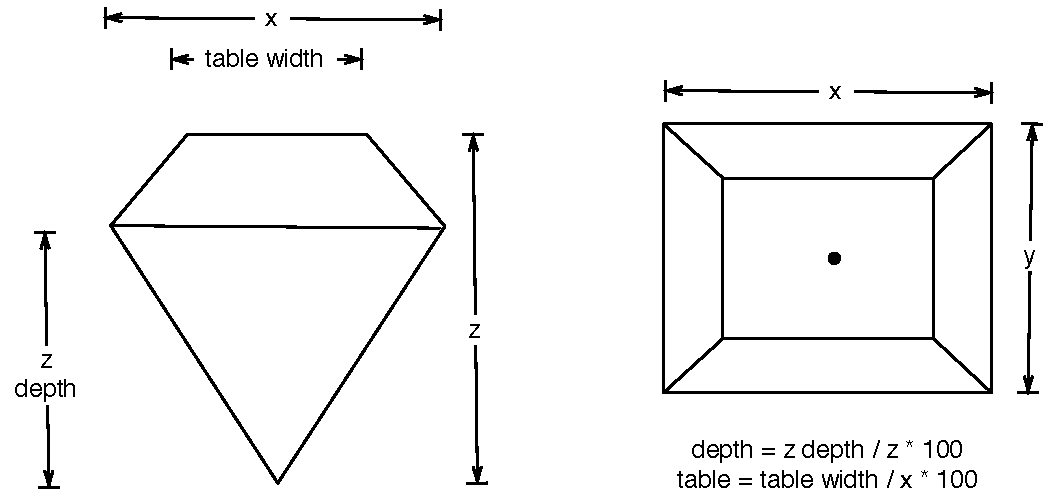
\includegraphics[width=0.8\linewidth]{diagrams/diamond-dimensions}
  \caption{How the variables x, y, z, table and depth are measured.}
  \label{fig:diamond-dim}
\end{figure}

The dataset has not been well cleaned, so as well as demonstrating
interesting relationships about diamonds, it also demonstrates some data
quality problems. We'll also use another dataset, \texttt{dsmall}, which
is a random sample of 100 diamonds. We'll use this data for plots that
are more appropriate for smaller datasets.

\begin{Shaded}
\begin{Highlighting}[]
\NormalTok{>}\StringTok{ }\KeywordTok{set.seed}\NormalTok{(}\DecValTok{1410}\NormalTok{) }\CommentTok{# Make the sample reproducible}
\NormalTok{>}\StringTok{ }\NormalTok{dsmall <-}\StringTok{ }\NormalTok{diamonds[}\KeywordTok{sample}\NormalTok{(}\KeywordTok{nrow}\NormalTok{(diamonds), }\DecValTok{100}\NormalTok{), ]}
\end{Highlighting}
\end{Shaded}

\hyperdef{}{sec:basic-use}{\section{Basic use}\label{sec:basic-use}}

As with \texttt{plot()}, the first two arguments to \texttt{qplot()} are
\texttt{x} and \texttt{y}, giving the x- and y-coordinates for the
objects on the plot. There is also an optional \texttt{data} argument.
If this is specified, \texttt{qplot()} will look inside that data frame
before looking for objects in your workspace. Using the \texttt{data}
argument is recommended: it's a good idea to keep related data in a
single data frame. If you don't specify one, \texttt{qplot()} will try
to build one up for you and may look in the wrong place.
\index{qplot!getting started} \indexf{qplot}

Here is a simple example of the use of \texttt{qplot()}. It produces a
scatterplot showing the relationship between the price and carats
(weight) of a diamond. \index{Scatterplot}

\begin{Shaded}
\begin{Highlighting}[]
\NormalTok{>}\StringTok{ }\KeywordTok{qplot}\NormalTok{(carat, price, }\DataTypeTok{data =} \NormalTok{diamonds)}
\end{Highlighting}
\end{Shaded}

\begin{flushleft}\includegraphics[width=0.49\linewidth]{figures/qplotqscatter-1} \end{flushleft}

The plot shows a strong correlation with notable outliers and some
interesting vertical striation. The relationship looks exponential,
though, so the first thing we'd like to do is to transform the
variables. Because \texttt{qplot()} accepts functions of variables as
arguments, we plot \texttt{log(price)} vs. \texttt{log(carat)}:

\begin{Shaded}
\begin{Highlighting}[]
\NormalTok{>}\StringTok{ }\KeywordTok{qplot}\NormalTok{(}\KeywordTok{log}\NormalTok{(carat), }\KeywordTok{log}\NormalTok{(price), }\DataTypeTok{data =} \NormalTok{diamonds)}
\end{Highlighting}
\end{Shaded}

\begin{flushleft}\includegraphics[width=0.49\linewidth]{figures/qplotqlog-1} \end{flushleft}

\noindent The relationship now looks linear. With this much
overplotting, though, we need to be cautious about drawing firm
conclusions.

Arguments can also be combinations of existing variables, so, if we are
curious about the relationship between the volume of the diamond
(approximated by \(x \times y \times z\)) and its weight, we could do
the following:

\begin{Shaded}
\begin{Highlighting}[]
\NormalTok{>}\StringTok{ }\KeywordTok{qplot}\NormalTok{(carat, x *}\StringTok{ }\NormalTok{y *}\StringTok{ }\NormalTok{z, }\DataTypeTok{data =} \NormalTok{diamonds)}
\end{Highlighting}
\end{Shaded}

\begin{flushleft}\includegraphics[width=0.49\linewidth]{figures/qplotvolume-1} \end{flushleft}

We would expect the density (weight/volume) of diamonds to be constant,
and so see a linear relationship between volume and weight. The majority
of diamonds do seem to fall along a line, but there are some large
outliers.

\hyperdef{}{sec:aesthetic-attributes}{\section{Colour, size, shape and
other aesthetic attributes}\label{sec:aesthetic-attributes}}

The first big difference when using \texttt{qplot()} instead of
\texttt{plot()} comes when you want to assign colours---or sizes or
shapes---to the points on your plot. With \texttt{plot()}, it's your
responsibility to convert a categorical variable in your data (e.g.,
`apples', `bananas', `pears') into something that \texttt{plot()} knows
how to use (e.g., `red', `yellow', `green'). \texttt{qplot()} can do
this for you automatically, and it will automatically provide a legend
that maps the displayed attributes to the data values. This makes it
easy to include additional data on the plot.

In the next example, we augment the plot of carat and price with
information about diamond colour and cut. The results are shown in
Figure \ref{fig:qplot-aesthetics}.

\begin{Shaded}
\begin{Highlighting}[]
\KeywordTok{qplot}\NormalTok{(carat, price, }\DataTypeTok{data =} \NormalTok{dsmall, }\DataTypeTok{colour =} \NormalTok{color)}
\KeywordTok{qplot}\NormalTok{(carat, price, }\DataTypeTok{data =} \NormalTok{dsmall, }\DataTypeTok{shape =} \NormalTok{cut)}
\end{Highlighting}
\end{Shaded}

\begin{figure}

{\centering \includegraphics[width=0.49\linewidth]{figures/qplotqplot-aesthetics-1} \includegraphics[width=0.49\linewidth]{figures/qplotqplot-aesthetics-2} 

}

\caption{Mapping point colour to diamond colour (left), and point shape to cut quality (right).\label{fig:qplot-aesthetics}}
\end{figure}

Colour, size and shape are all examples of aesthetic attributes, visual
properties that affect the way observations are displayed. For every
aesthetic attribute, there is a function, called a \emph{scale}, which
maps data values to valid values for that aesthetic. It is this scale
that controls the appearance of the points and associated legend. For
example, in the above plots, the colour scale maps J to purple and F to
green. (Note that while I use British spelling throughout this book, the
software also accepts American spellings.)\index{Aesthetics}

You can also manually set the aesthetics using \texttt{I()}, e.g.,
\texttt{colour = I("red")} or \texttt{size = I(2)}. This is not the same
as mapping and is explained in more detail in
\hyperref[sub:setting-mapping]{setting vs.~mapping}. For large datasets,
like the diamonds data, semi-transparent points are often useful to
alleviate some of the overplotting. To make a semi-transparent colour
you can use the alpha aesthetic, which takes a value between 0
(completely transparent) and 1 (complete opaque). It's often useful to
specify the transparency as a fraction, e.g., \texttt{1/10} or
\texttt{1/20}, as the denominator specifies the number of points that
must overplot to get a completely opaque colour.
\index{Aesthetics!setting} \indexf{I}

\begin{Shaded}
\begin{Highlighting}[]
\KeywordTok{qplot}\NormalTok{(carat, price, }\DataTypeTok{data =} \NormalTok{diamonds, }\DataTypeTok{alpha =} \KeywordTok{I}\NormalTok{(}\DecValTok{1}\NormalTok{/}\DecValTok{10}\NormalTok{))}
\KeywordTok{qplot}\NormalTok{(carat, price, }\DataTypeTok{data =} \NormalTok{diamonds, }\DataTypeTok{alpha =} \KeywordTok{I}\NormalTok{(}\DecValTok{1}\NormalTok{/}\DecValTok{100}\NormalTok{))}
\KeywordTok{qplot}\NormalTok{(carat, price, }\DataTypeTok{data =} \NormalTok{diamonds, }\DataTypeTok{alpha =} \KeywordTok{I}\NormalTok{(}\DecValTok{1}\NormalTok{/}\DecValTok{200}\NormalTok{))}
\end{Highlighting}
\end{Shaded}

\begin{figure}

{\centering \includegraphics[width=0.32\linewidth]{figures/qplotqplot-set-1} \includegraphics[width=0.32\linewidth]{figures/qplotqplot-set-2} \includegraphics[width=0.32\linewidth]{figures/qplotqplot-set-3} 

}

\caption{Reducing the alpha value from 1/10 (left) to 1/100 (middle) to 1/200 (right) makes it possible to see where the bulk of the points lie.\label{fig:qplot-set}}
\end{figure}

Different types of aesthetic attributes work better with different types
of variables. For example, colour and shape work well with categorical
variables, while size works better with continuous variables. The amount
of data also makes a difference: if there is a lot of data, like in the
plots above, it can be hard to distinguish the different groups. An
alternative solution is to use faceting (described in
\hyperref[sec:qplot-faceting]{link to section}).

\hyperdef{}{sec:plot-geoms}{\section{Plot geoms}\label{sec:plot-geoms}}

\texttt{qplot()} is not limited to scatterplots, but can produce almost
any kind of plot by varying the \texttt{geom} argument. Geom, short for
geometric object, describes the type of object that is used to display
the data. Some geoms have an associated statistical transformation, for
example, a histogram is a binning statistic plus a bar geom. These
different components are described in the next chapter. Here we'll
introduce the most common and useful geoms, organised by the
dimensionality of data that they work with. The following geoms enable
you to investigate two-dimensional relationships:

\begin{itemize}
\item
  \texttt{geom = "point"} draws points to produce a scatterplot. This is
  the default when you supply both \texttt{x} and \texttt{y} arguments
  to \texttt{qplot()}.
\item
  \texttt{geom = "smooth"} fits a smoother to the data and displays the
  smooth and its standard error, see \hyperref[sub:smooth]{adding a
  smoother to a plot}.
\item
  \texttt{geom = "boxplot"} produces a box-and-whisker plot to summarise
  the distribution of a set of points, see
  \hyperref[sub:boxplot]{boxplots and jittered points}.
\item
  \texttt{geom = "path"} and \texttt{geom = "line"} draw lines between
  the data points. Traditionally these are used to explore relationships
  between time and another variable, but lines may be used to join
  observations connected in some other way. A line plot is constrained
  to produce lines that travel from left to right, while paths can go in
  any direction, see \hyperref[sub:line]{time series with line and path
  plots}.
\end{itemize}

\noindent For 1d distributions, your choice of geoms is guided by the
variable type:

\begin{itemize}
\item
  For continuous variables, \texttt{geom = "histogram"} draws a
  histogram, \texttt{geom = "freqpoly"} a frequency polygon, and
  \texttt{geom = "density"} creates a density plot, see
  \hyperref[sub:distribution]{histogram and density plots}. The
  histogram geom is the default when you only supply an \texttt{x} value
  to \texttt{qplot()}.
\item
  For discrete variables, \texttt{geom = "bar"} makes a bar chart, see
  \hyperref[sub:bar]{bar charts}.
\end{itemize}

\hyperdef{}{sub:smooth}{\subsection{Adding a smoother to a
plot}\label{sub:smooth}}

If you have a scatterplot with many data points, it can be hard to see
exactly what trend is shown by the data. In this case you may want to
add a smoothed line to the plot. This is easily done using the
\texttt{smooth} geom as shown in Figure \ref{fig:qplot-smooth}. Notice
that we have combined multiple geoms by supplying a vector of geom names
created with \texttt{c()}. The geoms will be overlaid in the order in
which they appear. \index{Smoothing} \indexf{geom_smooth}

\begin{Shaded}
\begin{Highlighting}[]
\KeywordTok{qplot}\NormalTok{(carat, price, }\DataTypeTok{data =} \NormalTok{dsmall, }\DataTypeTok{geom =} \KeywordTok{c}\NormalTok{(}\StringTok{"point"}\NormalTok{, }\StringTok{"smooth"}\NormalTok{))}
\KeywordTok{qplot}\NormalTok{(carat, price, }\DataTypeTok{data =} \NormalTok{diamonds, }\DataTypeTok{geom =} \KeywordTok{c}\NormalTok{(}\StringTok{"point"}\NormalTok{, }\StringTok{"smooth"}\NormalTok{))}
\end{Highlighting}
\end{Shaded}

\begin{figure}

{\centering \includegraphics[width=0.49\linewidth]{figures/qplotqplot-smooth-1} \includegraphics[width=0.49\linewidth]{figures/qplotqplot-smooth-2} 

}

\caption{Smooth curves add to scatterplots of carat vs. price. The dsmall dataset (left) and the full dataset (right).\label{fig:qplot-smooth}}
\end{figure}

Despite overplotting, our impression of an exponential relationship
between price and carat was correct. There are few diamonds bigger than
three carats, and our uncertainty in the form of the relationship
increases as illustrated by the point-wise confidence interval shown in
grey. If you want to turn the confidence interval off, use
\texttt{se = FALSE}.

There are many different smoothers you can choose between by using the
\texttt{method} argument:

\begin{itemize}
\itemsep1pt\parskip0pt\parsep0pt
\item
  \texttt{method = "loess"}, the default for small n, uses a smooth
  local regression. More details about the algorithm used can be found
  in \texttt{?loess}. The wiggliness of the line is controlled by the
  \texttt{span} parameter, which ranges from 0 (exceedingly wiggly) to 1
  (not so wiggly), as shown in Figure \ref{fig:smooth-loess}.
  \index{Model!loess}
\end{itemize}

\begin{Shaded}
\begin{Highlighting}[]
\KeywordTok{qplot}\NormalTok{(carat, price, }\DataTypeTok{data =} \NormalTok{dsmall, }\DataTypeTok{geom =} \KeywordTok{c}\NormalTok{(}\StringTok{"point"}\NormalTok{, }\StringTok{"smooth"}\NormalTok{), }
  \DataTypeTok{span =} \FloatTok{0.2}\NormalTok{)}
\KeywordTok{qplot}\NormalTok{(carat, price, }\DataTypeTok{data =} \NormalTok{dsmall, }\DataTypeTok{geom =} \KeywordTok{c}\NormalTok{(}\StringTok{"point"}\NormalTok{, }\StringTok{"smooth"}\NormalTok{), }
  \DataTypeTok{span =} \DecValTok{1}\NormalTok{)}
\end{Highlighting}
\end{Shaded}

\begin{figure}

{\centering \includegraphics[width=0.49\linewidth]{figures/qplotsmooth-loess-1} \includegraphics[width=0.49\linewidth]{figures/qplotsmooth-loess-2} 

}

\caption{The effect of the span parameter.  (Left) \texttt{span = 0.2}, and (right) \texttt{span = 1}.\label{fig:smooth-loess}}
\end{figure}

\noindent Loess does not work well for large datasets (it's \(O(n^2)\)
in memory), and so an alternative smoothing algorithm is used when \(n\)
is greater than 1,000.

\begin{itemize}
\itemsep1pt\parskip0pt\parsep0pt
\item
  You could also load the \textbf{mgcv} library and use
  \texttt{method = "gam", formula = y \textasciitilde{} s(x)} to fit a
  generalised additive model. This is similar to using a spline with
  \texttt{lm()}, but the degree of smoothness is estimated from the
  data. For large data, use the formula
  \texttt{y \textasciitilde{} s(x, bs = "cs")}. This is used by default
  when there are more than 1,000 points. \index{Package!mgcv}
  \index{Model!generalised additive}
\end{itemize}

\begin{Shaded}
\begin{Highlighting}[]
\KeywordTok{library}\NormalTok{(mgcv)}
\KeywordTok{qplot}\NormalTok{(carat, price, }\DataTypeTok{data =} \NormalTok{dsmall, }\DataTypeTok{geom =} \KeywordTok{c}\NormalTok{(}\StringTok{"point"}\NormalTok{, }\StringTok{"smooth"}\NormalTok{), }
  \DataTypeTok{method =} \StringTok{"gam"}\NormalTok{, }\DataTypeTok{formula =} \NormalTok{y ~}\StringTok{ }\KeywordTok{s}\NormalTok{(x))}
\KeywordTok{qplot}\NormalTok{(carat, price, }\DataTypeTok{data =} \NormalTok{dsmall, }\DataTypeTok{geom =} \KeywordTok{c}\NormalTok{(}\StringTok{"point"}\NormalTok{, }\StringTok{"smooth"}\NormalTok{), }
  \DataTypeTok{method =} \StringTok{"gam"}\NormalTok{, }\DataTypeTok{formula =} \NormalTok{y ~}\StringTok{ }\KeywordTok{s}\NormalTok{(x, }\DataTypeTok{bs =} \StringTok{"cs"}\NormalTok{))}
\end{Highlighting}
\end{Shaded}

\begin{figure}

{\centering \includegraphics[width=0.49\linewidth]{figures/qplotsmooth-gam-1} \includegraphics[width=0.49\linewidth]{figures/qplotsmooth-gam-2} 

}

\caption{The effect of the formula parameter, using a generalised additive model as a smoother.  (Left) \texttt{formula = y \textasciitilde{} s(x)}, the default; (right) \texttt{formula = y \textasciitilde{} s(x, bs = 'cs')}.\label{fig:smooth-gam}}
\end{figure}

\begin{itemize}
\itemsep1pt\parskip0pt\parsep0pt
\item
  \texttt{method = "lm"} fits a linear model. The default will fit a
  straight line to your data, or you can specify
  \texttt{formula = y \textasciitilde{} poly(x, 2)} to specify a degree
  2 polynomial, or better, load the \textbf{splines} package and use a
  natural spline: \texttt{formula = y \textasciitilde{} ns(x, 2)}. The
  second parameter is the degrees of freedom: a higher number will
  create a wigglier curve. You are free to specify any formula involving
  \(x\) and \(y\). Figure \ref{fig:smooth-lm} shows two examples created
  with the following code. \index{Model!linear}
\end{itemize}

\begin{Shaded}
\begin{Highlighting}[]
\KeywordTok{library}\NormalTok{(splines)}
\KeywordTok{qplot}\NormalTok{(carat, price, }\DataTypeTok{data =} \NormalTok{dsmall, }\DataTypeTok{geom =} \KeywordTok{c}\NormalTok{(}\StringTok{"point"}\NormalTok{, }\StringTok{"smooth"}\NormalTok{), }
  \DataTypeTok{method =} \StringTok{"lm"}\NormalTok{)}
\KeywordTok{qplot}\NormalTok{(carat, price, }\DataTypeTok{data =} \NormalTok{dsmall, }\DataTypeTok{geom =} \KeywordTok{c}\NormalTok{(}\StringTok{"point"}\NormalTok{, }\StringTok{"smooth"}\NormalTok{), }
  \DataTypeTok{method =} \StringTok{"lm"}\NormalTok{, }\DataTypeTok{formula =} \NormalTok{y ~}\StringTok{ }\KeywordTok{ns}\NormalTok{(x, }\DecValTok{5}\NormalTok{))}
\end{Highlighting}
\end{Shaded}

\begin{figure}

{\centering \includegraphics[width=0.49\linewidth]{figures/qplotsmooth-lm-1} \includegraphics[width=0.49\linewidth]{figures/qplotsmooth-lm-2} 

}

\caption{The effect of the formula parameter, using a linear model as a smoother.  (Left) \texttt{formula = y \textasciitilde{} x}, the default; (right) \texttt{formula = y \textasciitilde{} ns(x, 5)}.\label{fig:smooth-lm}}
\end{figure}

\begin{itemize}
\itemsep1pt\parskip0pt\parsep0pt
\item
  \texttt{method = "rlm"} works like \texttt{lm()}, but uses a robust
  fitting algorithm so that outliers don't affect the fit as much. It's
  part of the \textbf{MASS} package, so remember to load that first.
  \index{Model!robust} \index{Package!MASS}
\end{itemize}

\hyperdef{}{sub:boxplot}{\subsection{Boxplots and jittered
points}\label{sub:boxplot}}

When a set of data includes a categorical variable and one or more
continuous variables, you will probably be interested to know how the
values of the continuous variables vary with the levels of the
categorical variable. Box-plots and jittered points offer two ways to do
this. Figure \ref{fig:jitter-boxplot} explores how the distribution of
price per carat varies with the colour of the diamond using jittering
(\texttt{geom = "jitter"}, left) and box-and-whisker plots
(\texttt{geom = "boxplot"}, right). \index{Boxplot} \index{Jittering}
\indexf{geom_boxplot}

\begin{Shaded}
\begin{Highlighting}[]
\KeywordTok{qplot}\NormalTok{(color, price /}\StringTok{ }\NormalTok{carat, }\DataTypeTok{data =} \NormalTok{diamonds, }\DataTypeTok{geom =} \StringTok{"jitter"}\NormalTok{)}
\KeywordTok{qplot}\NormalTok{(color, price /}\StringTok{ }\NormalTok{carat, }\DataTypeTok{data =} \NormalTok{diamonds, }\DataTypeTok{geom =} \StringTok{"boxplot"}\NormalTok{)}
\end{Highlighting}
\end{Shaded}

\begin{figure}

{\centering \includegraphics[width=0.49\linewidth]{figures/qplotjitter-boxplot-1} \includegraphics[width=0.49\linewidth]{figures/qplotjitter-boxplot-2} 

}

\caption{Using jittering (left) and boxplots (right) to investigate the distribution of price per carat, conditional on colour.  As the colour improves (from left to right) the spread of values decreases, but there is little change in the centre of the distribution.\label{fig:jitter-boxplot}}
\end{figure}

Each method has its strengths and weaknesses. Boxplots summarise the
bulk of the distribution with only five numbers, while jittered plots
show every point but can suffer from overplotting. In the example here,
both plots show the dependency of the spread of price per carat on
diamond colour, but the boxplots are more informative, indicating that
there is very little change in the median and adjacent quartiles.

The overplotting seen in the plot of jittered values can be alleviated
somewhat by using semi-transparent points using the \texttt{alpha}
argument. Figure \ref{fig:jitter-alpha} illustrates three different
levels of transparency, which make it easier to see where the bulk of
the points lie. The plots are produced with the following code.
\indexf{geom_jitter}

\begin{Shaded}
\begin{Highlighting}[]
\KeywordTok{qplot}\NormalTok{(color, price /}\StringTok{ }\NormalTok{carat, }\DataTypeTok{data =} \NormalTok{diamonds, }\DataTypeTok{geom =} \StringTok{"jitter"}\NormalTok{,}
 \DataTypeTok{alpha =} \KeywordTok{I}\NormalTok{(}\DecValTok{1} \NormalTok{/}\StringTok{ }\DecValTok{5}\NormalTok{))}
\KeywordTok{qplot}\NormalTok{(color, price /}\StringTok{ }\NormalTok{carat, }\DataTypeTok{data =} \NormalTok{diamonds, }\DataTypeTok{geom =} \StringTok{"jitter"}\NormalTok{,}
 \DataTypeTok{alpha =} \KeywordTok{I}\NormalTok{(}\DecValTok{1} \NormalTok{/}\StringTok{ }\DecValTok{50}\NormalTok{))}
\KeywordTok{qplot}\NormalTok{(color, price /}\StringTok{ }\NormalTok{carat, }\DataTypeTok{data =} \NormalTok{diamonds, }\DataTypeTok{geom =} \StringTok{"jitter"}\NormalTok{,}
 \DataTypeTok{alpha =} \KeywordTok{I}\NormalTok{(}\DecValTok{1} \NormalTok{/}\StringTok{ }\DecValTok{200}\NormalTok{))}
\end{Highlighting}
\end{Shaded}

\begin{figure}

{\centering \includegraphics[width=0.32\linewidth]{figures/qplotjitter-alpha-1} \includegraphics[width=0.32\linewidth]{figures/qplotjitter-alpha-2} \includegraphics[width=0.32\linewidth]{figures/qplotjitter-alpha-3} 

}

\caption{Varying the alpha level.  From left to right: $1/5$, $1/50$, $1/200$.  As the opacity decreases we begin to see where the bulk of the data lies.  However, the boxplot still does much better.\label{fig:jitter-alpha}}
\end{figure}

This technique can't show the positions of the quantiles as well as a
boxplot can, but it may reveal other features of the distribution that a
boxplot cannot.

For jittered points, \texttt{qplot()} offers the same control over
aesthetics as it does for a normal scatterplot: \texttt{size},
\texttt{colour} and \texttt{shape}. For boxplots you can control the
outline \texttt{colour}, the internal \texttt{fill} colour and the
\texttt{size} of the lines.

Another way to look at conditional distributions is to use faceting
(described in \hyperref[sec:qplot-faceting]{link to section}) to plot a
separate histogram or density plot for each value of the categorical
variable.

\hyperdef{}{sub:distribution}{\subsection{Histogram and density
plots}\label{sub:distribution}}

Histogram and density plots show the distribution of a single variable.
They provide more information about the distribution of a single group
than boxplots do, but it is harder to compare many groups (although we
will look at one way to do so). Figure \ref{fig:dist} shows the
distribution of carats with a histogram and a density plot.
\index{Histogram} \index{Density!plot} \indexf{geom_histogram}
\indexf{geom_density}

\begin{Shaded}
\begin{Highlighting}[]
\KeywordTok{qplot}\NormalTok{(carat, }\DataTypeTok{data =} \NormalTok{diamonds, }\DataTypeTok{geom =} \StringTok{"histogram"}\NormalTok{)}
\KeywordTok{qplot}\NormalTok{(carat, }\DataTypeTok{data =} \NormalTok{diamonds, }\DataTypeTok{geom =} \StringTok{"density"}\NormalTok{)}
\end{Highlighting}
\end{Shaded}

\begin{figure}

{\centering \includegraphics[width=0.49\linewidth]{figures/qplotdist-1} \includegraphics[width=0.49\linewidth]{figures/qplotdist-2} 

}

\caption{Displaying the distribution of diamonds.  (Left) \texttt{geom = 'histogram'} and (right) \texttt{geom = 'density'}.\label{fig:dist}}
\end{figure}

For the density plot, the \texttt{adjust} argument controls the degree
of smoothness (high values of \texttt{adjust} produce smoother plots).
For the histogram, the \texttt{binwidth} argument controls the amount of
smoothing by setting the bin size. (Break points can also be specified
explicitly, using the \texttt{breaks} argument.) It is \textbf{very
important} to experiment with the level of smoothing. With a histogram
you should try many bin widths: You may find that gross features of the
data show up well at a large bin width, while finer features require a
very narrow width.

In Figure \ref{fig:hist-binwidth}, we experiment with three values of
\texttt{binwidth}: 1.0, 0.1 and 0.01. It is only in the plot with the
smallest bin width (right) that we see the striations we noted in an
earlier scatterplot, most at `nice' numbers of carats. The full code is:

\begin{Shaded}
\begin{Highlighting}[]
\KeywordTok{qplot}\NormalTok{(carat, }\DataTypeTok{data =} \NormalTok{diamonds, }\DataTypeTok{geom =} \StringTok{"histogram"}\NormalTok{, }\DataTypeTok{binwidth =} \DecValTok{1}\NormalTok{, }
  \DataTypeTok{xlim =} \KeywordTok{c}\NormalTok{(}\DecValTok{0}\NormalTok{,}\DecValTok{3}\NormalTok{))}
\KeywordTok{qplot}\NormalTok{(carat, }\DataTypeTok{data =} \NormalTok{diamonds, }\DataTypeTok{geom =} \StringTok{"histogram"}\NormalTok{, }\DataTypeTok{binwidth =} \FloatTok{0.1}\NormalTok{,}
  \DataTypeTok{xlim =} \KeywordTok{c}\NormalTok{(}\DecValTok{0}\NormalTok{,}\DecValTok{3}\NormalTok{))}
\KeywordTok{qplot}\NormalTok{(carat, }\DataTypeTok{data =} \NormalTok{diamonds, }\DataTypeTok{geom =} \StringTok{"histogram"}\NormalTok{, }\DataTypeTok{binwidth =} \FloatTok{0.01}\NormalTok{,}
  \DataTypeTok{xlim =} \KeywordTok{c}\NormalTok{(}\DecValTok{0}\NormalTok{,}\DecValTok{3}\NormalTok{))}
\end{Highlighting}
\end{Shaded}

\begin{figure}

{\centering \includegraphics[width=0.32\linewidth]{figures/qplothist-binwidth-1} \includegraphics[width=0.32\linewidth]{figures/qplothist-binwidth-2} \includegraphics[width=0.32\linewidth]{figures/qplothist-binwidth-3} 

}

\caption{Varying the bin width on a histogram of carat reveals interesting patterns.  Binwidths from left to right: 1, 0.1 and 0.01 carats. Only diamonds between 0 and 3 carats shown.\label{fig:hist-binwidth}}
\end{figure}

To compare the distributions of different subgroups, just add an
aesthetic mapping, as in the following code.

\begin{Shaded}
\begin{Highlighting}[]
\KeywordTok{qplot}\NormalTok{(carat, }\DataTypeTok{data =} \NormalTok{diamonds, }\DataTypeTok{geom =} \StringTok{"density"}\NormalTok{, }\DataTypeTok{colour =} \NormalTok{color)}
\KeywordTok{qplot}\NormalTok{(carat, }\DataTypeTok{data =} \NormalTok{diamonds, }\DataTypeTok{geom =} \StringTok{"histogram"}\NormalTok{, }\DataTypeTok{fill =} \NormalTok{color)}
\end{Highlighting}
\end{Shaded}

\begin{figure}

{\centering \includegraphics[width=0.49\linewidth]{figures/qplotdist-fill-1} \includegraphics[width=0.49\linewidth]{figures/qplotdist-fill-2} 

}

\caption{Mapping a categorical variable to an aesthetic will automatically split up the geom by that variable.  (Left) Density plots are overlaid and (right) histograms are stacked.\label{fig:dist-fill}}
\end{figure}

\noindent Mapping a categorical variable to an aesthetic will
automatically split up the geom by that variable, so these commands
instruct \texttt{qplot()} to draw a density plot and histogram for each
level of diamond colour. The results are shown in Figure
\ref{fig:dist-fill}.

The density plot is more appealing at first because it seems easy to
read and compare the various curves. However, it is more difficult to
understand exactly what a density plot is showing. In addition, the
density plot makes some assumptions that may not be true for our data;
i.e., that it is unbounded, continuous and smooth.

\hyperdef{}{sub:bar}{\subsection{Bar charts}\label{sub:bar}}

The discrete analogue of histogram is the bar chart,
\texttt{geom = "bar"}. The bar geom counts the number of instances of
each class so that you don't need to tabulate your values beforehand, as
with \texttt{barplot()} in base R. If the data has already been
tabulated or if you'd like to tabulate class members in some other way,
such as by summing up a continuous variable, you can use the
\texttt{weight} geom. This is illustrated in Figure \ref{fig:dist-bar}.
The first plot is a simple bar chart of diamond colour, and the second
is a bar chart of diamond colour weighted by carat. \index{Barchart}
\indexf{geom_bar}

\begin{Shaded}
\begin{Highlighting}[]
\KeywordTok{qplot}\NormalTok{(color, }\DataTypeTok{data =} \NormalTok{diamonds, }\DataTypeTok{geom =} \StringTok{"bar"}\NormalTok{)}
\KeywordTok{qplot}\NormalTok{(color, }\DataTypeTok{data =} \NormalTok{diamonds, }\DataTypeTok{geom =} \StringTok{"bar"}\NormalTok{, }\DataTypeTok{weight =} \NormalTok{carat) +}
\StringTok{  }\KeywordTok{scale_y_continuous}\NormalTok{(}\StringTok{"carat"}\NormalTok{)}
\end{Highlighting}
\end{Shaded}

\begin{figure}

{\centering \includegraphics[width=0.49\linewidth]{figures/qplotdist-bar-1} \includegraphics[width=0.49\linewidth]{figures/qplotdist-bar-2} 

}

\caption{Bar charts of diamond colour.  The left plot shows counts and the right plot is weighted by \texttt{weight = carat} to show the total weight of diamonds of each colour.\label{fig:dist-bar}}
\end{figure}

\hyperdef{}{sub:line}{\subsection{Time series with line and path
plots}\label{sub:line}}

Line and path plots are typically used for time series data. Line plots
join the points from left to right, while path plots join them in the
order that they appear in the dataset (a line plot is just a path plot
of the data sorted by x value). Line plots usually have time on the
x-axis, showing how a single variable has changed over time. Path plots
show how two variables have simultaneously changed over time, with time
encoded in the way that the points are joined together.

Because there is no time variable in the diamonds data, we use the
\texttt{economics} dataset, which contains economic data on the US
measured over the last 40 years. Figure \ref{fig:line-employment} shows
two plots of unemployment over time, both produced using
\texttt{geom = "line"}. The first shows an unemployment rate and the
second shows the median number of weeks unemployed. We can already see
some differences in these two variables, particularly in the last peak,
where the unemployment percentage is lower than it was in the preceding
peaks, but the length of unemployment is high.
\index{Time series!bivariate} \indexf{geom_line} \indexf{geom_path}

\begin{Shaded}
\begin{Highlighting}[]
\KeywordTok{qplot}\NormalTok{(date, unemploy /}\StringTok{ }\NormalTok{pop, }\DataTypeTok{data =} \NormalTok{economics, }\DataTypeTok{geom =} \StringTok{"line"}\NormalTok{)}
\KeywordTok{qplot}\NormalTok{(date, uempmed, }\DataTypeTok{data =} \NormalTok{economics, }\DataTypeTok{geom =} \StringTok{"line"}\NormalTok{)}
\end{Highlighting}
\end{Shaded}

\begin{figure}

{\centering \includegraphics[width=0.49\linewidth]{figures/qplotline-employment-1} \includegraphics[width=0.49\linewidth]{figures/qplotline-employment-2} 

}

\caption{Two time series measuring amount of unemployment.  (Left) Proportion of population that is unemployed and (right) median number of weeks unemployed.  Plots created with \texttt{geom='line'}.\label{fig:line-employment}}
\end{figure}

To examine this relationship in greater detail, we would like to draw
both time series on the same plot. We could draw a scatterplot of
unemployment rate vs.~length of unemployment, but then we could no
longer see the evolution over time. The solution is to join points
adjacent in time with line segments, forming a \emph{path} plot.

Below we plot unemployment rate vs.~length of unemployment and join the
individual observations with a path. Because of the many line crossings,
the direction in which time flows isn't easy to see in the first plot.
In the second plot, we apply the \texttt{colour} aesthetic to the line
to make it easier to see the direction of time.

\begin{Shaded}
\begin{Highlighting}[]
\NormalTok{year <-}\StringTok{ }\NormalTok{function(x) }\KeywordTok{as.POSIXlt}\NormalTok{(x)$year +}\StringTok{ }\DecValTok{1900}
\KeywordTok{qplot}\NormalTok{(unemploy /}\StringTok{ }\NormalTok{pop, uempmed, }\DataTypeTok{data =} \NormalTok{economics, }
   \DataTypeTok{geom =} \KeywordTok{c}\NormalTok{(}\StringTok{"point"}\NormalTok{, }\StringTok{"path"}\NormalTok{))}
\KeywordTok{qplot}\NormalTok{(unemploy /}\StringTok{ }\NormalTok{pop, uempmed, }\DataTypeTok{data =} \NormalTok{economics, }
  \DataTypeTok{geom =} \StringTok{"path"}\NormalTok{, }\DataTypeTok{colour =} \KeywordTok{year}\NormalTok{(date))}
\end{Highlighting}
\end{Shaded}

\begin{figure}

{\centering \includegraphics[width=0.49\linewidth]{figures/qplotpath-employ-1} \includegraphics[width=0.49\linewidth]{figures/qplotpath-employ-2} 

}

\caption{Path plots illustrating the relationship between percent of people unemployed and median length of unemployment.  (Left) Scatterplot with overlaid path.  (Right) Pure path plot coloured by year.\label{fig:path-employ}}
\end{figure}

We can see that percent unemployed and length of unemployment are highly
correlated, although in recent years the length of unemployment has been
increasing relative to the unemployment rate.

With longitudinal data, you often want to display multiple time series
on each plot, each series representing one individual. To do this with
\texttt{qplot()}, you need to map the \texttt{group} aesthetic to a
variable encoding the group membership of each observation. This is
explained in more depth in \hyperref[sub:grouping]{grouping}.
\index{Longitudinal data|see{Time series}} \index{Data!longitudinal}

\hyperdef{}{sec:qplot-faceting}{\section{Faceting}\label{sec:qplot-faceting}}

We have already discussed using aesthetics (colour and shape) to compare
subgroups, drawing all groups on the same plot. Faceting takes an
alternative approach: It creates tables of graphics by splitting the
data into subsets and displaying the same graph for each subset in an
arrangement that facilitates comparison.
\hyperref[sec:faceting]{Faceting} discusses faceting in detail,
including a discussion of the advantages and disadvantages of using
faceting instead of aesthetics in \hyperref[sub:group-vs-facet]{grouping
vs.~faceting}. \index{Faceting}

The default faceting method in \texttt{qplot()} creates plots arranged
on a grid specified by a faceting formula which looks like
\texttt{row\_var \textasciitilde{} col\_var}. You can specify as many
row and column variables as you like, keeping in mind that using more
than two variables will often produce a plot so large that it is
difficult to see on screen. To facet on only one of columns or rows, use
\texttt{.} as a place holder. For example,
\texttt{row\_var \textasciitilde{} .} will create a single column with
multiple rows. \indexf{facet_grid}

Figure \ref{fig:facet-hist} illustrates this technique with two plots,
sets of histograms showing the distribution of carat conditional on
colour. The second set of histograms shows proportions, making it easier
to compare distributions regardless of the relative abundance of
diamonds of each colour. The \texttt{..density..} syntax is new. The
y-axis of the histogram does not come from the original data, but from
the statistical transformation that counts the number of observations in
each bin. Using \texttt{..density..} tells \textbf{ggplot} to map the
density to the y-axis instead of the default use of count.

\begin{Shaded}
\begin{Highlighting}[]
\KeywordTok{qplot}\NormalTok{(carat, }\DataTypeTok{data =} \NormalTok{diamonds, }\DataTypeTok{facets =} \NormalTok{color ~}\StringTok{ }\NormalTok{., }
  \DataTypeTok{geom =} \StringTok{"histogram"}\NormalTok{, }\DataTypeTok{binwidth =} \FloatTok{0.1}\NormalTok{, }\DataTypeTok{xlim =} \KeywordTok{c}\NormalTok{(}\DecValTok{0}\NormalTok{, }\DecValTok{3}\NormalTok{))}
\KeywordTok{qplot}\NormalTok{(carat, ..density.., }\DataTypeTok{data =} \NormalTok{diamonds, }\DataTypeTok{facets =} \NormalTok{color ~}\StringTok{ }\NormalTok{.,}
  \DataTypeTok{geom =} \StringTok{"histogram"}\NormalTok{, }\DataTypeTok{binwidth =} \FloatTok{0.1}\NormalTok{, }\DataTypeTok{xlim =} \KeywordTok{c}\NormalTok{(}\DecValTok{0}\NormalTok{, }\DecValTok{3}\NormalTok{))}
\end{Highlighting}
\end{Shaded}

\begin{figure}

{\centering \includegraphics[width=0.49\linewidth]{figures/qplotfacet-hist-1} \includegraphics[width=0.49\linewidth]{figures/qplotfacet-hist-2} 

}

\caption{Histograms showing the distribution of carat conditional on colour.  (Left) Bars show counts and (right) bars show densities (proportions of the whole).  The density plot makes it easier to compare distributions ignoring the relative abundance of diamonds within each colour. High-quality diamonds (colour D) are skewed towards small sizes, and as quality declines the distribution becomes more flat.\label{fig:facet-hist}}
\end{figure}

\hyperdef{}{sec:other-options}{\section{Other
options}\label{sec:other-options}}

These are a few other \texttt{qplot()} options to control the graphic's
appearance. These all have the same effect as their \texttt{plot()}
equivalents: \index{qplot!other options}

\begin{itemize}
\itemsep1pt\parskip0pt\parsep0pt
\item
  \texttt{xlim}, \texttt{ylim}: set limits for the x- and y-axes, each a
  numeric vector of length two, e.g., \texttt{xlim=c(0, 20)} or
  \texttt{ylim=c(-0.9, -0.5)}. \index{Axis!limits}
\item
  \texttt{log}: a character vector indicating which (if any) axes should
  be logged. For example, \texttt{log="x"} will log the x-axis,
  \texttt{log="xy"} will log both.\index{Log transform}
\item
  \texttt{main}: main title for the plot, centered in large text at the
  top of the plot. This can be a string (e.g.,
  \texttt{main="plot title"}) or an expression (e.g.,
  \texttt{main = expression(beta{[}1{]} == 1)}). See \texttt{?plotmath}
  for more examples of using mathematical formulae. \index{Title}
\item
  \texttt{xlab}, \texttt{ylab}: labels for the x- and y-axes. As with
  the plot title, these can be character strings or mathematical
  expressions. \index{Axis!labels}
\end{itemize}

The following examples show the options in action.

\begin{Shaded}
\begin{Highlighting}[]
\NormalTok{>}\StringTok{ }\KeywordTok{qplot}\NormalTok{(}
\NormalTok{+}\StringTok{   }\NormalTok{carat, price, }\DataTypeTok{data =} \NormalTok{dsmall, }
\NormalTok{+}\StringTok{   }\DataTypeTok{xlab =} \StringTok{"Weight (carats)"}\NormalTok{, }\DataTypeTok{ylab =} \StringTok{"Price ($)"}\NormalTok{,}
\NormalTok{+}\StringTok{   }\DataTypeTok{main =} \StringTok{"Price-weight relationship"}
\NormalTok{+}\StringTok{ }\NormalTok{)}
\end{Highlighting}
\end{Shaded}

\begin{flushleft}\includegraphics[width=0.4\linewidth]{figures/qplotlabels-1} \end{flushleft}

\begin{Shaded}
\begin{Highlighting}[]
\NormalTok{>}\StringTok{ }\KeywordTok{qplot}\NormalTok{(}
\NormalTok{+}\StringTok{    }\NormalTok{carat, price/carat, }\DataTypeTok{data =} \NormalTok{dsmall, }
\NormalTok{+}\StringTok{    }\DataTypeTok{ylab =} \KeywordTok{expression}\NormalTok{(}\KeywordTok{frac}\NormalTok{(price,carat)), }
\NormalTok{+}\StringTok{    }\DataTypeTok{xlab =} \StringTok{"Weight (carats)"}\NormalTok{,  }
\NormalTok{+}\StringTok{    }\DataTypeTok{main =} \StringTok{"Small diamonds"}\NormalTok{, }
\NormalTok{+}\StringTok{    }\DataTypeTok{xlim =} \KeywordTok{c}\NormalTok{(.}\DecValTok{2}\NormalTok{,}\DecValTok{1}\NormalTok{)}
\NormalTok{+}\StringTok{ }\NormalTok{)}
\end{Highlighting}
\end{Shaded}

\begin{flushleft}\includegraphics[width=0.4\linewidth]{figures/qplotlabels-2} \end{flushleft}

\begin{Shaded}
\begin{Highlighting}[]
\NormalTok{>}\StringTok{ }\KeywordTok{qplot}\NormalTok{(carat, price, }\DataTypeTok{data =} \NormalTok{dsmall, }\DataTypeTok{log =} \StringTok{"xy"}\NormalTok{)}
\end{Highlighting}
\end{Shaded}

\begin{flushleft}\includegraphics[width=0.4\linewidth]{figures/qplotlabels-3} \end{flushleft}

\hyperdef{}{sec:plot-diffs}{\section{Differences from
plot}\label{sec:plot-diffs}}

There are a few important differences between \texttt{plot()} and
\texttt{qplot()}:
\index{qplot!differences from plot@differences from \texttt{plot()}}
\indexf{plot}

\begin{itemize}
\item
  \texttt{qplot()} is not generic: you cannot pass any type of R object
  to qplot and expect to get some kind of default plot. Note, however,
  that \texttt{ggplot()} is generic, and may provide a starting point
  for producing visualisations of arbitrary R objects. See
  \hyperref[cha:data]{data} for more details.
\item
  Usually you will supply a variable to the aesthetic attribute you're
  interested in. This is then scaled and displayed with a legend. If you
  want to set the value, e.g., to make red points, use \texttt{I()}:
  \texttt{colour = I("red")}. This is explained in more detail in
  \hyperref[sub:setting-mapping]{setting vs.~mapping}.
\item
  While you can continue to use the base R aesthetic names
  (\texttt{col}, \texttt{pch}, \texttt{cex}, etc.), it's a good idea to
  switch to the more descriptive \textbf{ggplot} aesthetic names
  (\texttt{colour}, \texttt{shape} and \texttt{size}). They're much
  easier to remember!
\item
  To add further graphic elements to a plot produced in base graphics,
  you can use \texttt{points()}, \texttt{lines()} and \texttt{text()}.
  With \textbf{ggplot2}, you need to add additional \textbf{layers} to
  the existing plot, described in the next chapter.
\end{itemize}
